\chapter{Test Journal: DC motor inductance $\boldsymbol{L_a}$ and resistance $\boldsymbol{R_a}$}
\label{test:DC-motorFrequencySweep}
\begin{table}[!h]
\begin{tabular}{l l}
\textbf{Test participants:} & Maxime \& Robin  \\
\textbf{Date:}  & 12/10-2016
\end{tabular}
\end{table}

\section*{Purpose}
The purpose of the test is to determine the internal inductance and resistance of the DC motor. This is done by running a frequency sweep through the motor and measuring the response while its rotor shaft locked.

\section*{Test equipment and components}
The test equipment and components are listed in \autoref{tab_appendix:DC-motorFrequencySweepComponents}.
\begin{table}[h]
	\centering
	\caption{List of measurement equipment and components}\label{tab_appendix:DC-motorFrequencySweepComponents}

	\begin{tabularx}{\textwidth}{l X X X X}
		Name 				& Brand	& Model & AAU-number\\ \toprule \rowcolor{lightGrey}
		PC & Fujistu Siemens Computers & MI3W-D2312 & 64640 \\
		DC motor & Maxon & 41.023.038-00.00-052& N/A \\ \rowcolor{lightGrey}
		$\SI{20.1}{\ohm}$ resistor & N/A & N/A & N/A \\
	\end{tabularx}
\end{table}

\section*{Setup}
The measurement setup is seen on \autoref{fig:DCFrequencySweepSetup}.

%\begin{figure} [h!]
%	\centering
%	\begin{subfigure}{0.4\textwidth}
%		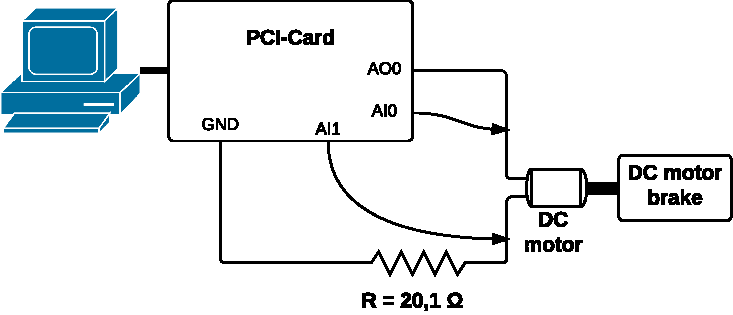
\includegraphics [width=\textwidth]{figures/test/DCR_circuit}
%		\caption{Circuit diagram}
%		\label{fig:DCFrequencySweepSetupDiagram}
%	\end{subfigure}
%	~ 
%	\begin{subfigure}{0.4\textwidth}
%		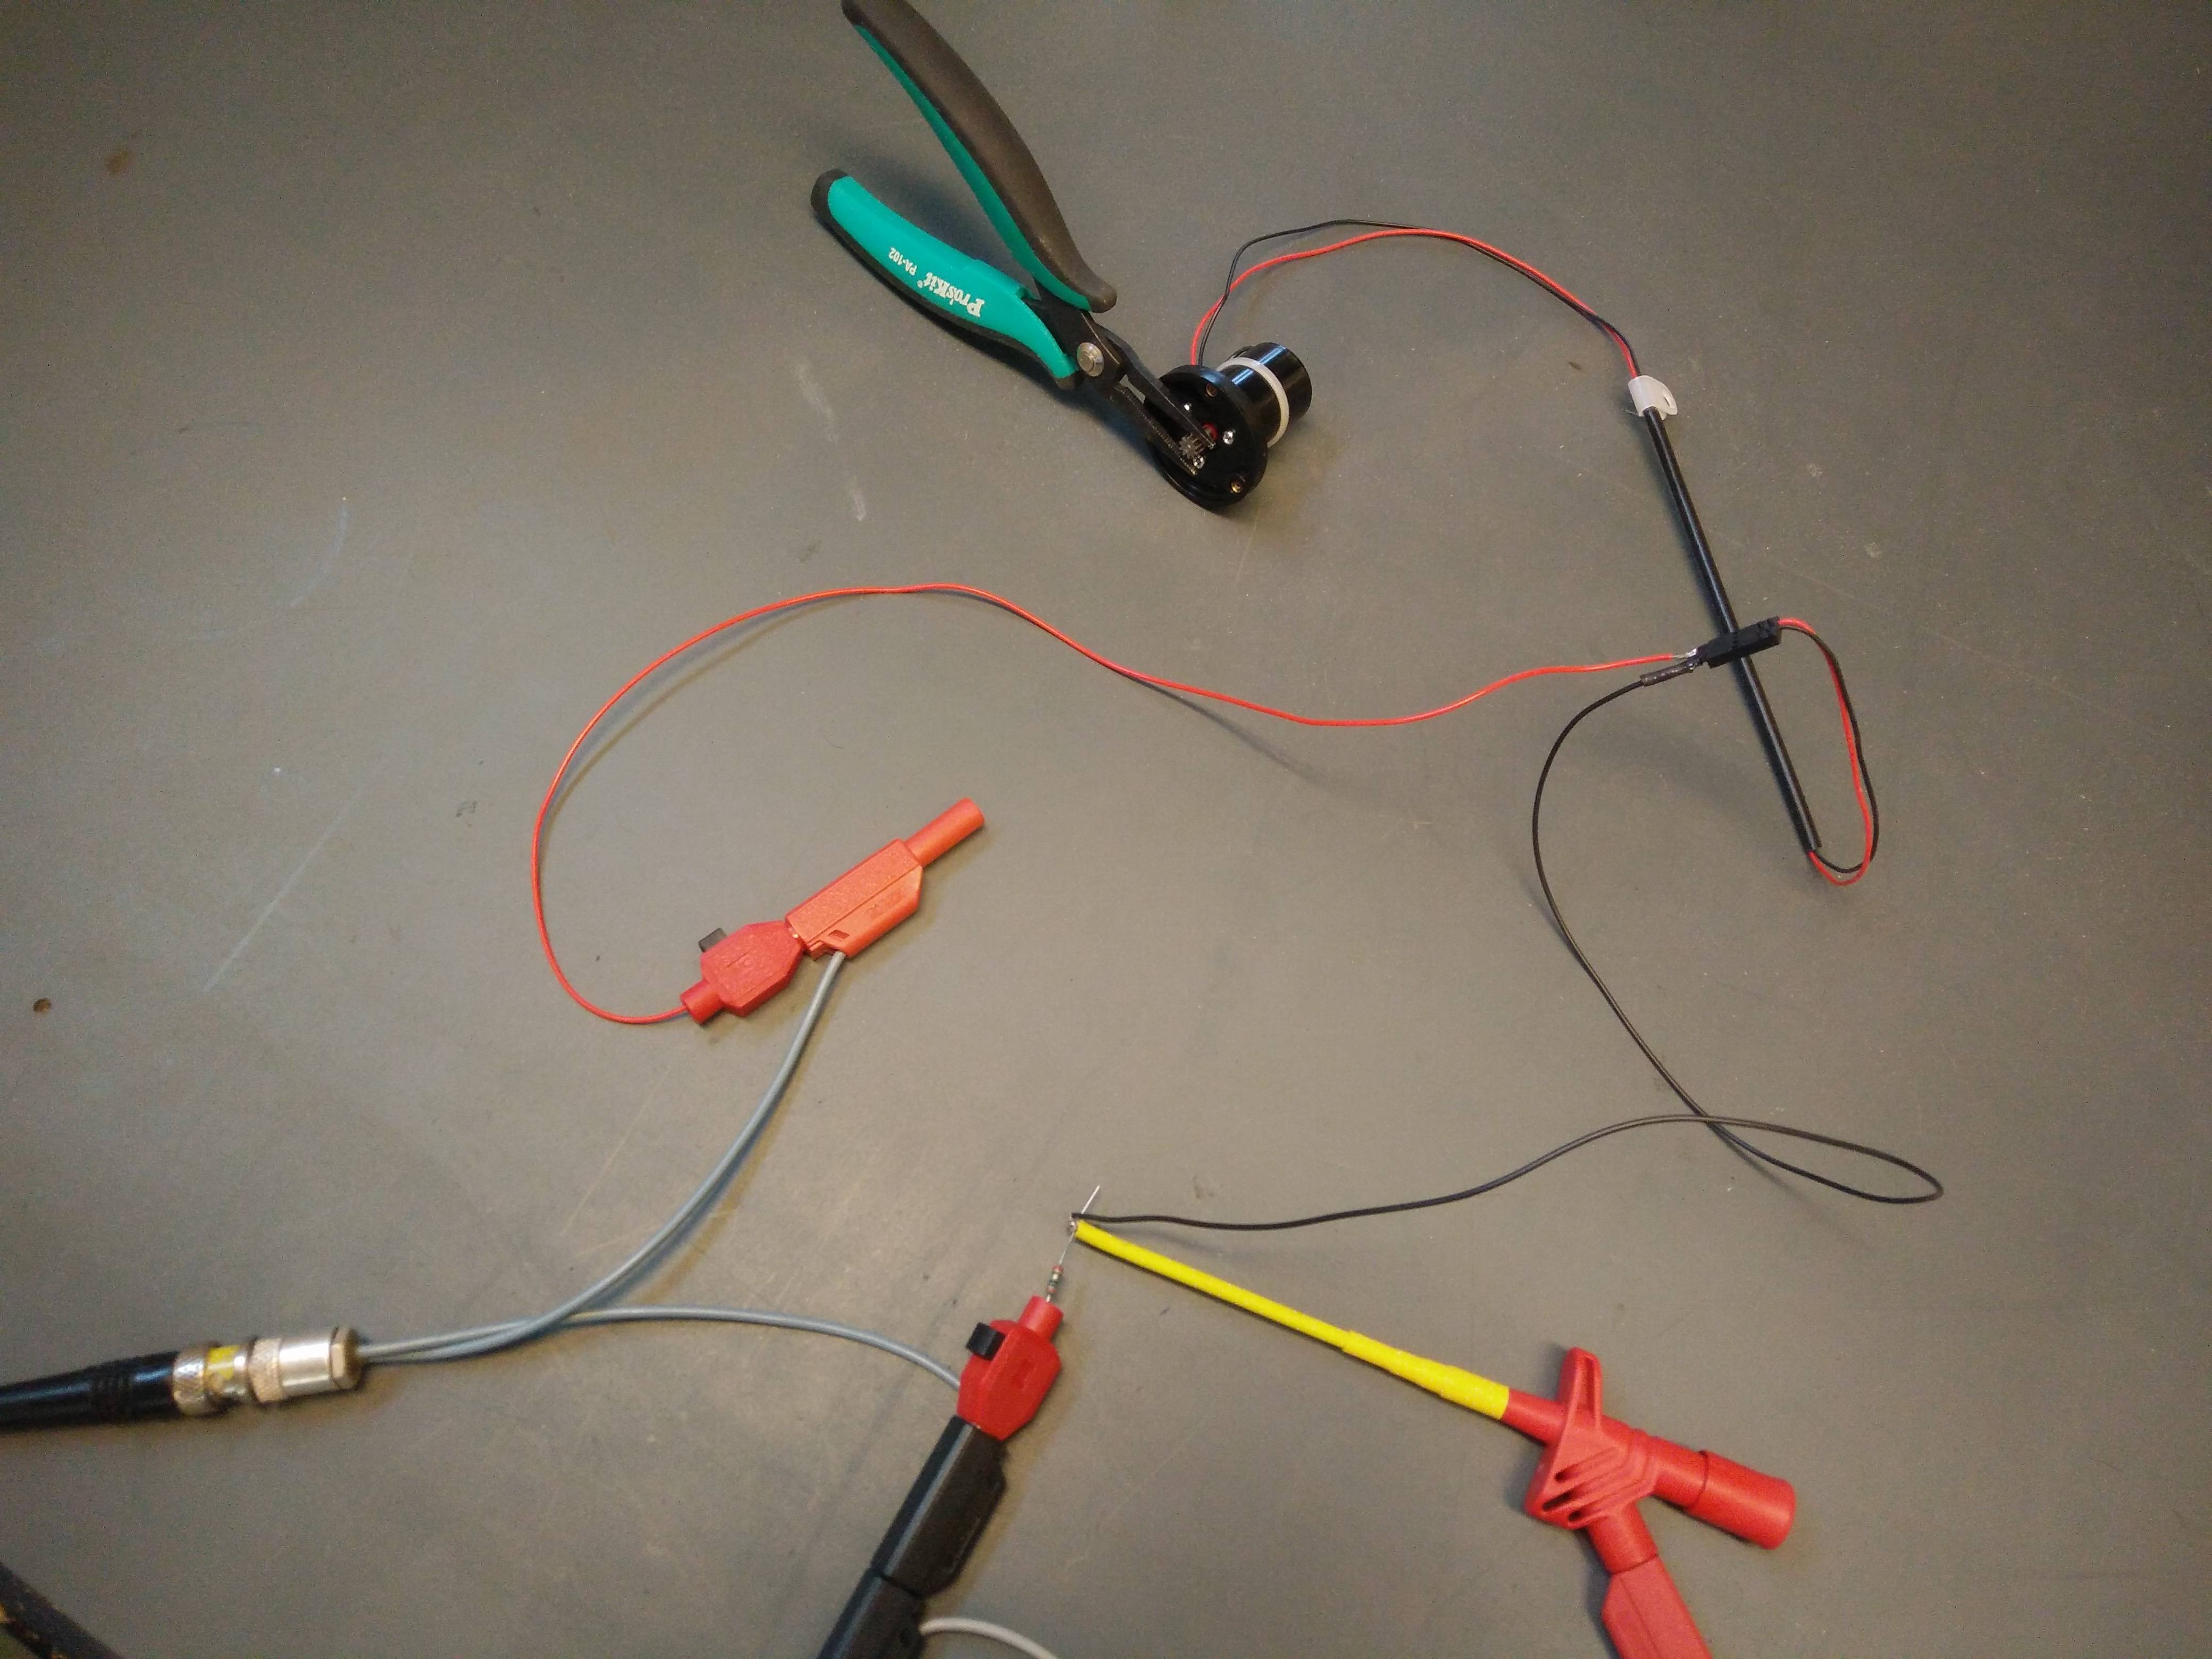
\includegraphics[width=\textwidth]{figures/test/FrequencySweepTest.jpg}
%		\caption{Real set-up}
%		\label{fig:DCFrequencySweepSetupR}
%	\end{subfigure}
%	\caption{Measurement setup}\label{fig:DCFrequencySweepSetup}
%\end{figure}
\begin{figure}
\centering
		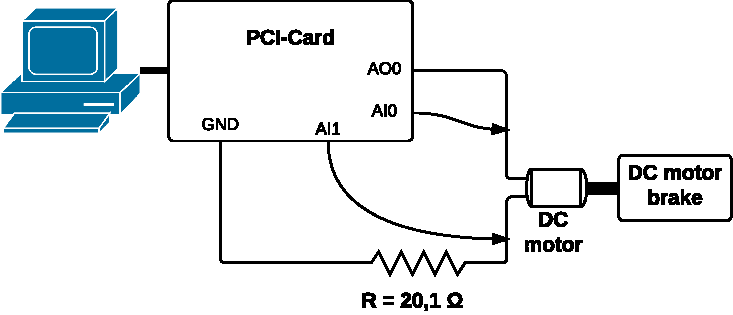
\includegraphics [width=0.75\textwidth]{figures/test/DCR_circuit}
		\caption{Measurement setup diagram.}
		\label{fig:DCFrequencySweepSetup}
	\end{figure}
This circuit is wired to the PC through the NI-4461 PCI-card that handles the frequency sweep.

\section*{Method}
The DC motor, in series with a resistor is connected to the NI-4461 PCI-card as illustrated on \autoref{fig:DCFrequencySweepSetup}. The setup allows the PC to measure the incoming signal through $\texttt{AI0}$ and the voltage across the known resistor, through $\texttt{AI1}$.  

The PC is set to run a frequency sweep with an amplitude of \SI{1}{\volt}, from \SI{0}{\hertz} to \SI{24}{\kilo\hertz} in 200 steps, with a sampling frequency of \SI{50}{\kilo\hertz}.
%\todo[author=Daniel, inline]{Include position of the "sweet wires" on the figure. Were did you put the cables to the sweep PC?}

\section*{Results}
The results from the frequency sweep, as well as the calculated response are illustrated on \ref{fig:DCFrequencySweepRawData} .

\begin{figure}
	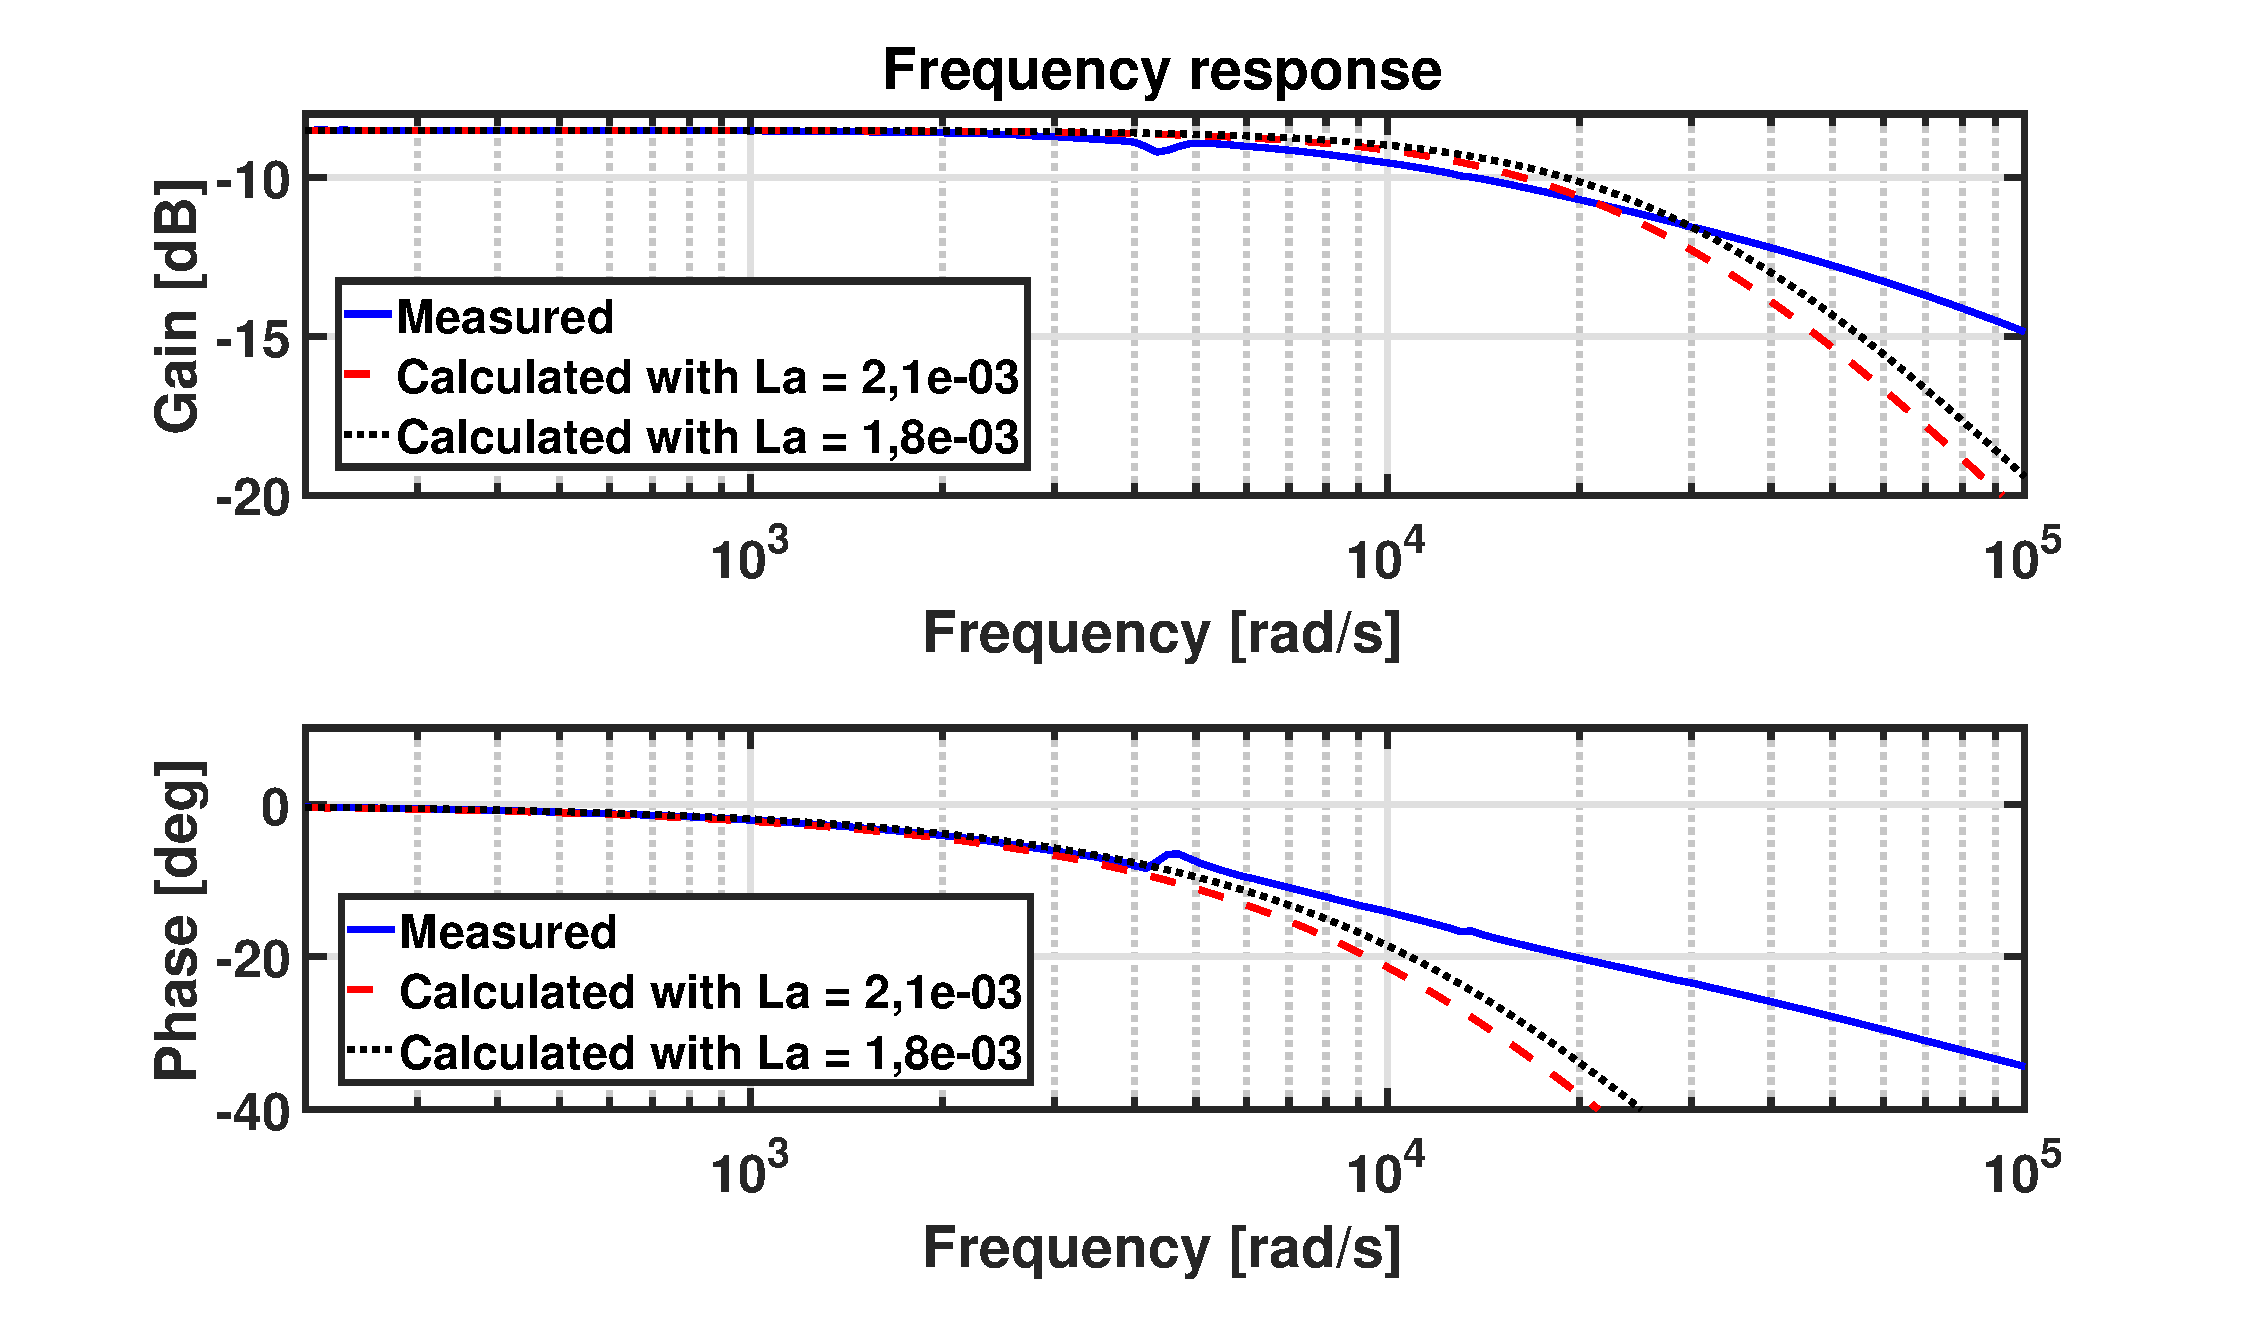
\includegraphics[width = \textwidth]{figures/test/DCFrequencySweepRaw.eps}
	\caption{Plot of the frequency response of the DC motor. The measured and two calculated responses are illustrated.}
	\label{fig:DCFrequencySweepRawData}
\end{figure}

\section*{Data processing}
The voltage across DC motor and resistor can be expressed in the laplace domain as \autoref{appendix:eq:sweepVoltage}.
\begin{equation} 
V_{i}(s) = V_{s}(s) + V_r(s) \label{appendix:eq:sweepVoltage}
\end{equation}
\startexplain
\explain{$V_i(s)$ is the voltage across the resistor and motor}{\si{\volt}}
\explain{$V_s(s)$ is the voltage across the motor}{\si{\volt}}
\explain{$V_r(s)$ is the voltage across the resistor}{\si{\volt}}
\stopexplain

\autoref{eq:DC-motorElecEq} describes the expected behaviour of the DC motor. When the DC motors rotor shaft is locked, the equation can be written as \autoref{appendix:eq:sweepMotorTranfsferFunction}, assuming initial conditions are zero.
\begin{equation} 
V_{s}(s) = R_{a}\cdot I_a(s) + I_a(s)\cdot s\cdot L_a \label{appendix:eq:sweepMotorTranfsferFunction}
\end{equation}

The current can be expressed in relation to the voltage across the resistor as in \autoref{appendix:eq:sweepResistorVoltage}
\begin{equation} 
I_{a}(s) = \frac{V_r(s)}{R} \label{appendix:eq:sweepResistorVoltage}
\end{equation}

Combining Equations \ref{appendix:eq:sweepVoltage}, \ref{appendix:eq:sweepMotorTranfsferFunction} and \ref{appendix:eq:sweepResistorVoltage}, nets \autoref{appendix:eq:sweepTF}
\begin{equation} 
V_i(s) = R_a \frac{V_r(s)}{R} + \frac{V_r(s)}{R} \cdot s \cdot L_a + V_r(s) \implies \frac{V_r(s)}{V_i(s)} = H(s) = \frac{\frac{R}{L_a}}{s+\frac{R+R_a}{L_a}} \label{appendix:eq:sweepTF}
\end{equation}

From \autoref{appendix:eq:sweepTF} one can derive that $H (0) = \frac{R}{R_a+R}$ and that there is a pole at $0 = s + \frac{R+R_a}{L_a}$.
Using these observations, $L_a$ and $R_a$ can be calculated by Equations \ref{DC-motorLaEq} and \ref{DC-motorRaEq}.
\begin{equation}
	\omega_{3dB} = \frac{R+R_a}{L_a} \implies L_a = \frac{R_a+R}{\omega_{3dB}}
	\label{DC-motorLaEq}
\end{equation}
\startexplain
\explain{$\omega_{3dB}$ is the corner frequency where the gain is \SI{-3}{\deci\bel}}{\si{\volt}}
\stopexplain
\begin{equation}
	R_a = \frac{R}{H (0)}-R
	\label{DC-motorRaEq}
\end{equation}

Using Equations \ref{DC-motorLaEq} and \ref{DC-motorRaEq}, the inductance and resistance can be calculated in Equations \ref{DC-motorFinalEqR} and \ref{DC-motorFinalEqL}.
\begin{subequations}
	\begin{align}
	&\notag R = \SI{20.1}{\ohm}\\
	&H (0) = 10^{-\frac{8.52}{20}}  =\frac{R}{R_a+R} \implies R_a = \SI{33.5}{\ohm}\label{DC-motorFinalEqR}\\
	&\omega_{3dB} = 2\cdot\pi\cdot 4741 = \frac{R+R_a}{L_a}  \implies L_a = \SI{1.8}{\milli\henry}
	&\label{DC-motorFinalEqL}
	\end{align}
\end{subequations}

It is however through trail and error seen that an inductance $L_a=\SI{2.1}{\milli\henry}$ is a better fit at lower frequencies, as illustrated on \autoref{fig:DCFrequencySweepRawData}. $L_a=\SI{2.1}{\milli\henry}$ is therefore chosen for the model.

\section*{Conclusion}
\begin{table}[h!]
	\centering
	\caption{Summery of the results of the tests.}
\begin{tabular}{llll}
\textit{Component}	&	\textit{Symbol} &  	\textit{Value} &  \textit{Unit} \\ \rowcolor{lightGrey} \toprule
Resistance				&	$R_a$	& \SI{33.5}{} 			   & $\SI{}{\ohm}$ \\
Inductance				&	$L_a$	& \SI{2.1}{}			   & $\SI{}{\milli\henry}$ 
\end{tabular}\label{tab:Dc-motorconst}
\end{table}
		
		